\begin{frame}
\frametitle{Optimizations}
\framesubtitle{Stages}
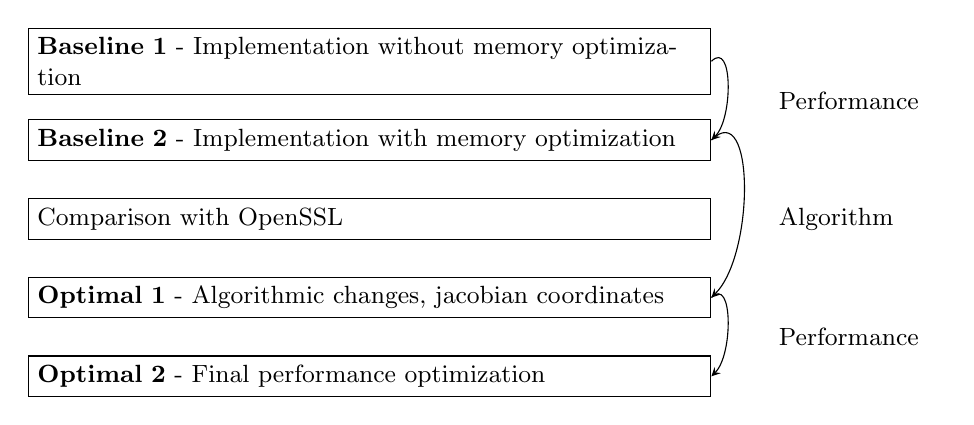
\begin{tikzpicture}[
rect/.style={
draw,
text width=24em,
},
myedge/.style={
out=45,
in=45,
->,
>=stealth,
},
font=\small,
scale = 0.5
]
\node[rect] at (0,8) (1) {\textbf{Baseline 1} - Implementation without memory optimization};
\node[rect] at (0,6) (2) {\textbf{Baseline 2} - Implementation with memory optimization};
\node[rect] at (0,4) (3) {Comparison with OpenSSL};
\node[rect] at (0,2) (4) {\textbf{Optimal 1} - Algorithmic changes, jacobian coordinates};
\node[rect] at (0,0) (5) {\textbf{Optimal 2} - Final performance optimization };


\path (1.east) edge [myedge] (2.east);
\path (2.east) edge [myedge] (4.east);
\path (4.east) edge [myedge] (5.east);

\node[text width=2cm] at (12.4,7) {Performance };
\node[text width=2cm] at (12.4,4) {Algorithm };
\node[text width=2cm] at (12.4,1) {Performance };

\end{tikzpicture}
\end{frame}

\begin{frame}[fragile]
\frametitle{Intel ADX}
C Code
\begin{lstlisting}[frame=single, basicstyle=\tiny]
low_m1 = _mulx_u64(a->blocks[i], b, &hi_m1); 
add_carry_m1 = _addcarryx_u64(add_carry_m1, carry_m1, low_m1, &temp_m1);
add_carry_1 = _addcarryx_u64(add_carry_1, res->blocks[i], temp_m1, tmp->blocks[i]);
carry_m1 = hi_m1;
\end{lstlisting}
Created Assembly code\\
x86 icc 13.0.1 -m64 -march=haswell -O3
\begin{lstlisting}[frame=single, basicstyle=\tiny, language={[x86masm]Assembler}]
mov       rdx, QWORD PTR [48+rsi]
mulx      rdx, rbx, rax
adox      rbp, rdx
adcx      rbp, QWORD PTR [48+rdi]
mov       QWORD PTR [2288+r9], rbp 
\end{lstlisting}
\vfill
\tiny{http://gcc.godbolt.org/}
\end{frame}

\begin{frame}[fragile]
\frametitle{Intel ADX}
C Code
\begin{lstlisting}[frame=single, basicstyle=\tiny]
low_m1 = _mulx_u64(a->blocks[i], b, &hi_m1); 
add_carry_m1 = _addcarryx_u64(add_carry_m1, carry_m1, low_m1, &temp_m1);
add_carry_1 = _addcarryx_u64(add_carry_1, res->blocks[i], temp_m1, tmp->blocks[i]);
carry_m1 = hi_m1;
\end{lstlisting}
Created Assembly code\\
x86 gcc 5.3 -m64 -march=haswell -O3
\begin{lstlisting}[frame=single, basicstyle=\tiny, language={[x86masm]Assembler}]
mulx    48(%rsi), %r9, %r10
addq    %r9, %r11
movq    %r10, %r9
setc    %bpl
addb    $-1, %bl
adcq    48(%rdi), %r11
movq    %r11, 2288(%rax)
setc    %bl
addb    $-1, %bpl
\end{lstlisting}
\vfill
\tiny{http://gcc.godbolt.org/}
\end{frame}

%\begin{frame}
%  \frametitle{Vectorization}
%  \begin{tikzpicture}[scale=0.55]
%  \draw (0,0) -- (3,0) -- (3,1) -- (0,1) -- (0,0);
%  \draw (3,0) -- (6,0) -- (6,1) -- (3,1);
%  \draw (6,0) -- (9,0) -- (9,1) -- (6,1);
%  \draw (9,0) -- (12,0) -- (12,1) -- (9,1);
%  
%  \node[minimum width=0.5cm] at (1.5,1.5) {+};
%  \node[minimum width=0.5cm,] at (4.5,1.5) {+};
%  \node[minimum width=0.5cm,] at (7.5,1.5) {+};
%  %\node[minimum width=0.5cm,] at (10.5,1.5) {+};
%  
%  \node[minimum width=0.5cm,] at (4.5,2.5) {$b_2$};
%  \node[minimum width=0.5cm,] at (7.5,2.5) {$b_1$};
%  \node[minimum width=0.5cm,] at (10.5,2.5) {$b_0$};
%  
%  \draw (0,2) -- (3,2) -- (3,3) -- (0,3) -- (0,2);
%  \draw (3,2) -- (6,2) -- (6,3) -- (3,3);
%  \draw (6,2) -- (9,2) -- (9,3) -- (6,3);
%  \draw (9,2) -- (12,2) -- (12,3) -- (9,3);
%  
%  %\node[minimum width=0.5cm,align=center] at (1.5,3.5) {+};
%  \node[minimum width=0.5cm,] at (4.5,3.5) {+};
%  \node[minimum width=0.5cm,] at (7.5,3.5) {+};
%  \node[minimum width=0.5cm,] at (10.5,3.5) {+};
%  
%  \node[minimum width=0.5cm,] at (4.5,4.5) {$a_2$};
%  \node[minimum width=0.5cm,] at (7.5,4.5) {$a_1$};
%  \node[minimum width=0.5cm,] at (10.5,4.5) {$a_0$};
%  
%  \draw (0,4) -- (3,4) -- (3,5) -- (0,5) -- (0,4);
%  \draw (3,4) -- (6,4) -- (6,5) -- (3,5);
%  \draw (6,4) -- (9,4) -- (9,5) -- (6,5);
%  \draw (9,4) -- (12,4) -- (12,5) -- (9,5);
%  
%  \draw[arrows=->,line width=.4pt](10.5, 2)--(7.5,1);
%  \draw[arrows=->,line width=.4pt](7.5, 2)--(4.5,1);
%  \draw[arrows=->,line width=.4pt](4.5, 2)--(1.5,1);
%  
%  \node[text width=0.5cm,align=left] at (12.5,4.5) {LSB};
%  \node[text width=0.5cm,align=left] at (12.5,2.5) {LSB};
%  \node[text width=0.5cm,align=left] at (12.5,0.5) {LSB};
%  
%  \node[text width=3.5cm,align=left] at (17.5,4.5) {$a = \sum_{i=0}^{2} a_i \left(2^{64}\right)^i$};
%  \node[text width=3.5cm,align=left] at (17.5,2.5) {$b = \sum_{i=0}^{2} b_i \left(2^{64}\right)^i$};
%  \node[text width=3.5cm,align=left] at (17.5,0.5) {carry};
%  \end{tikzpicture}
%\end{frame}